\section{Results}

The three SLAM algorithms were evaluated regarding the computed trajectories, the resulting point clouds and
the computational cost. 


\fig{img/perc_seq.png}{Boxplot of the percentages of the sequences, that were tracked by the algorithm for each run.}{fig:percseq}{1}

Each algorithm needs a certain time to start the tracking. For example, when the drone rests at the first ten seconds of the sequence, the SLAM 
algorithm will not be able to initialize, since it needs a transformation to recognize the position of a point or feature in space. The amount of required transformations 
is needed is algorithm-specific. Also, as discussed in section \ref{complement}, ORB SLAM3 provides the possibility to create a new local map, once the tracking
was lost and merge the new map with the old one, when the places from the old map are revisited within the new map. However, if the tracking is lost and hence 
a new map is created, but no places from the old map are revisited, these maps can not be merged. Therefore it is possible to yield multiple maps for 
a single sequence. In case this happens, only the map with the largest amount of keyframes is considered, and the resulting trajectory and point cloud is derived
from this respective map only. In figure \ref{fig:percseq} the percentages of the sequences where the tracking was successful are displayed. For most sequences, 
the percentage is similar between the algorithms and the runs. Small differences underlie the differences of the end time-point of the initialization process. However, 
for sequences V103 and V203, ORB SLAM created a second map, that could not be merged with the old one. Hence, for one run in sequence V103 and for all runs in 
sequence V203, a part of the tracking is missing. This needs to be taken into consideration when analyzing the results. 

The fact, that in one run the tracking can be lost, while within the same algorithm and sequence the tracking is not lost in another run, suggests the 
conclusion that runs within the same algorithm and same sequence can yield different results. The confirmation of the conclusion is displayed in figures 
\ref{fig:comp2} and \ref{fig:comp1}. 

\fig{img/comp_runs2.png}{Distances to the ground truth position for the trajectory of all runs within an algorithm for sequence MH01}{fig:comp2}{1}

The first figure shows the results of all runs for the sequence MH01, which is an easy sequence to track, since the the velocity of the drone and the 
angular velocity is low, while the sequence provides a bright scene and good texture. Differences between the runs for the sequence are not large, but they exist. 
For example the first run of ORB SLAM needs more time to initialize the tracking, which causes the tracking to start later and end earlier. These differences between runs
may result from the fact, that the algorithms run in different threads, that perform simultaneously. This does not guarantee that the computations always occur in the same succession. 
Differences seem to be lower for DSO SLAM. This may be because DSO SLAM has no thread performing global optimization simultaneously. 

\fig{img/comp_runs_V203.png}{Distances to the ground truth position for the trajectory of all runs within an algorithm for sequence V203}{fig:comp1}{1}

For more difficult sequences, that might even cause some runs to loose tracking while others don't, as it can be seen in figure \ref{fig:comp1}

\subsection{Trajectory Evaluation}

	After alignment, as a first indicator for the accuracy of the computed trajectories, the trajectories were visually investigated by 
	plotting the true position and the evaluated position into a coordinate system. This method 
    for comparing the trajectories is described in detail in section \ref{poseval}. Obviously, those trajectories, that align perfectly with the ground truth
	suggest that the position was correctly evaluated by the algorithm. 
	
	% and here 

	\begin{figure}%
    \centering
    \subfloat[\centering MH01]{{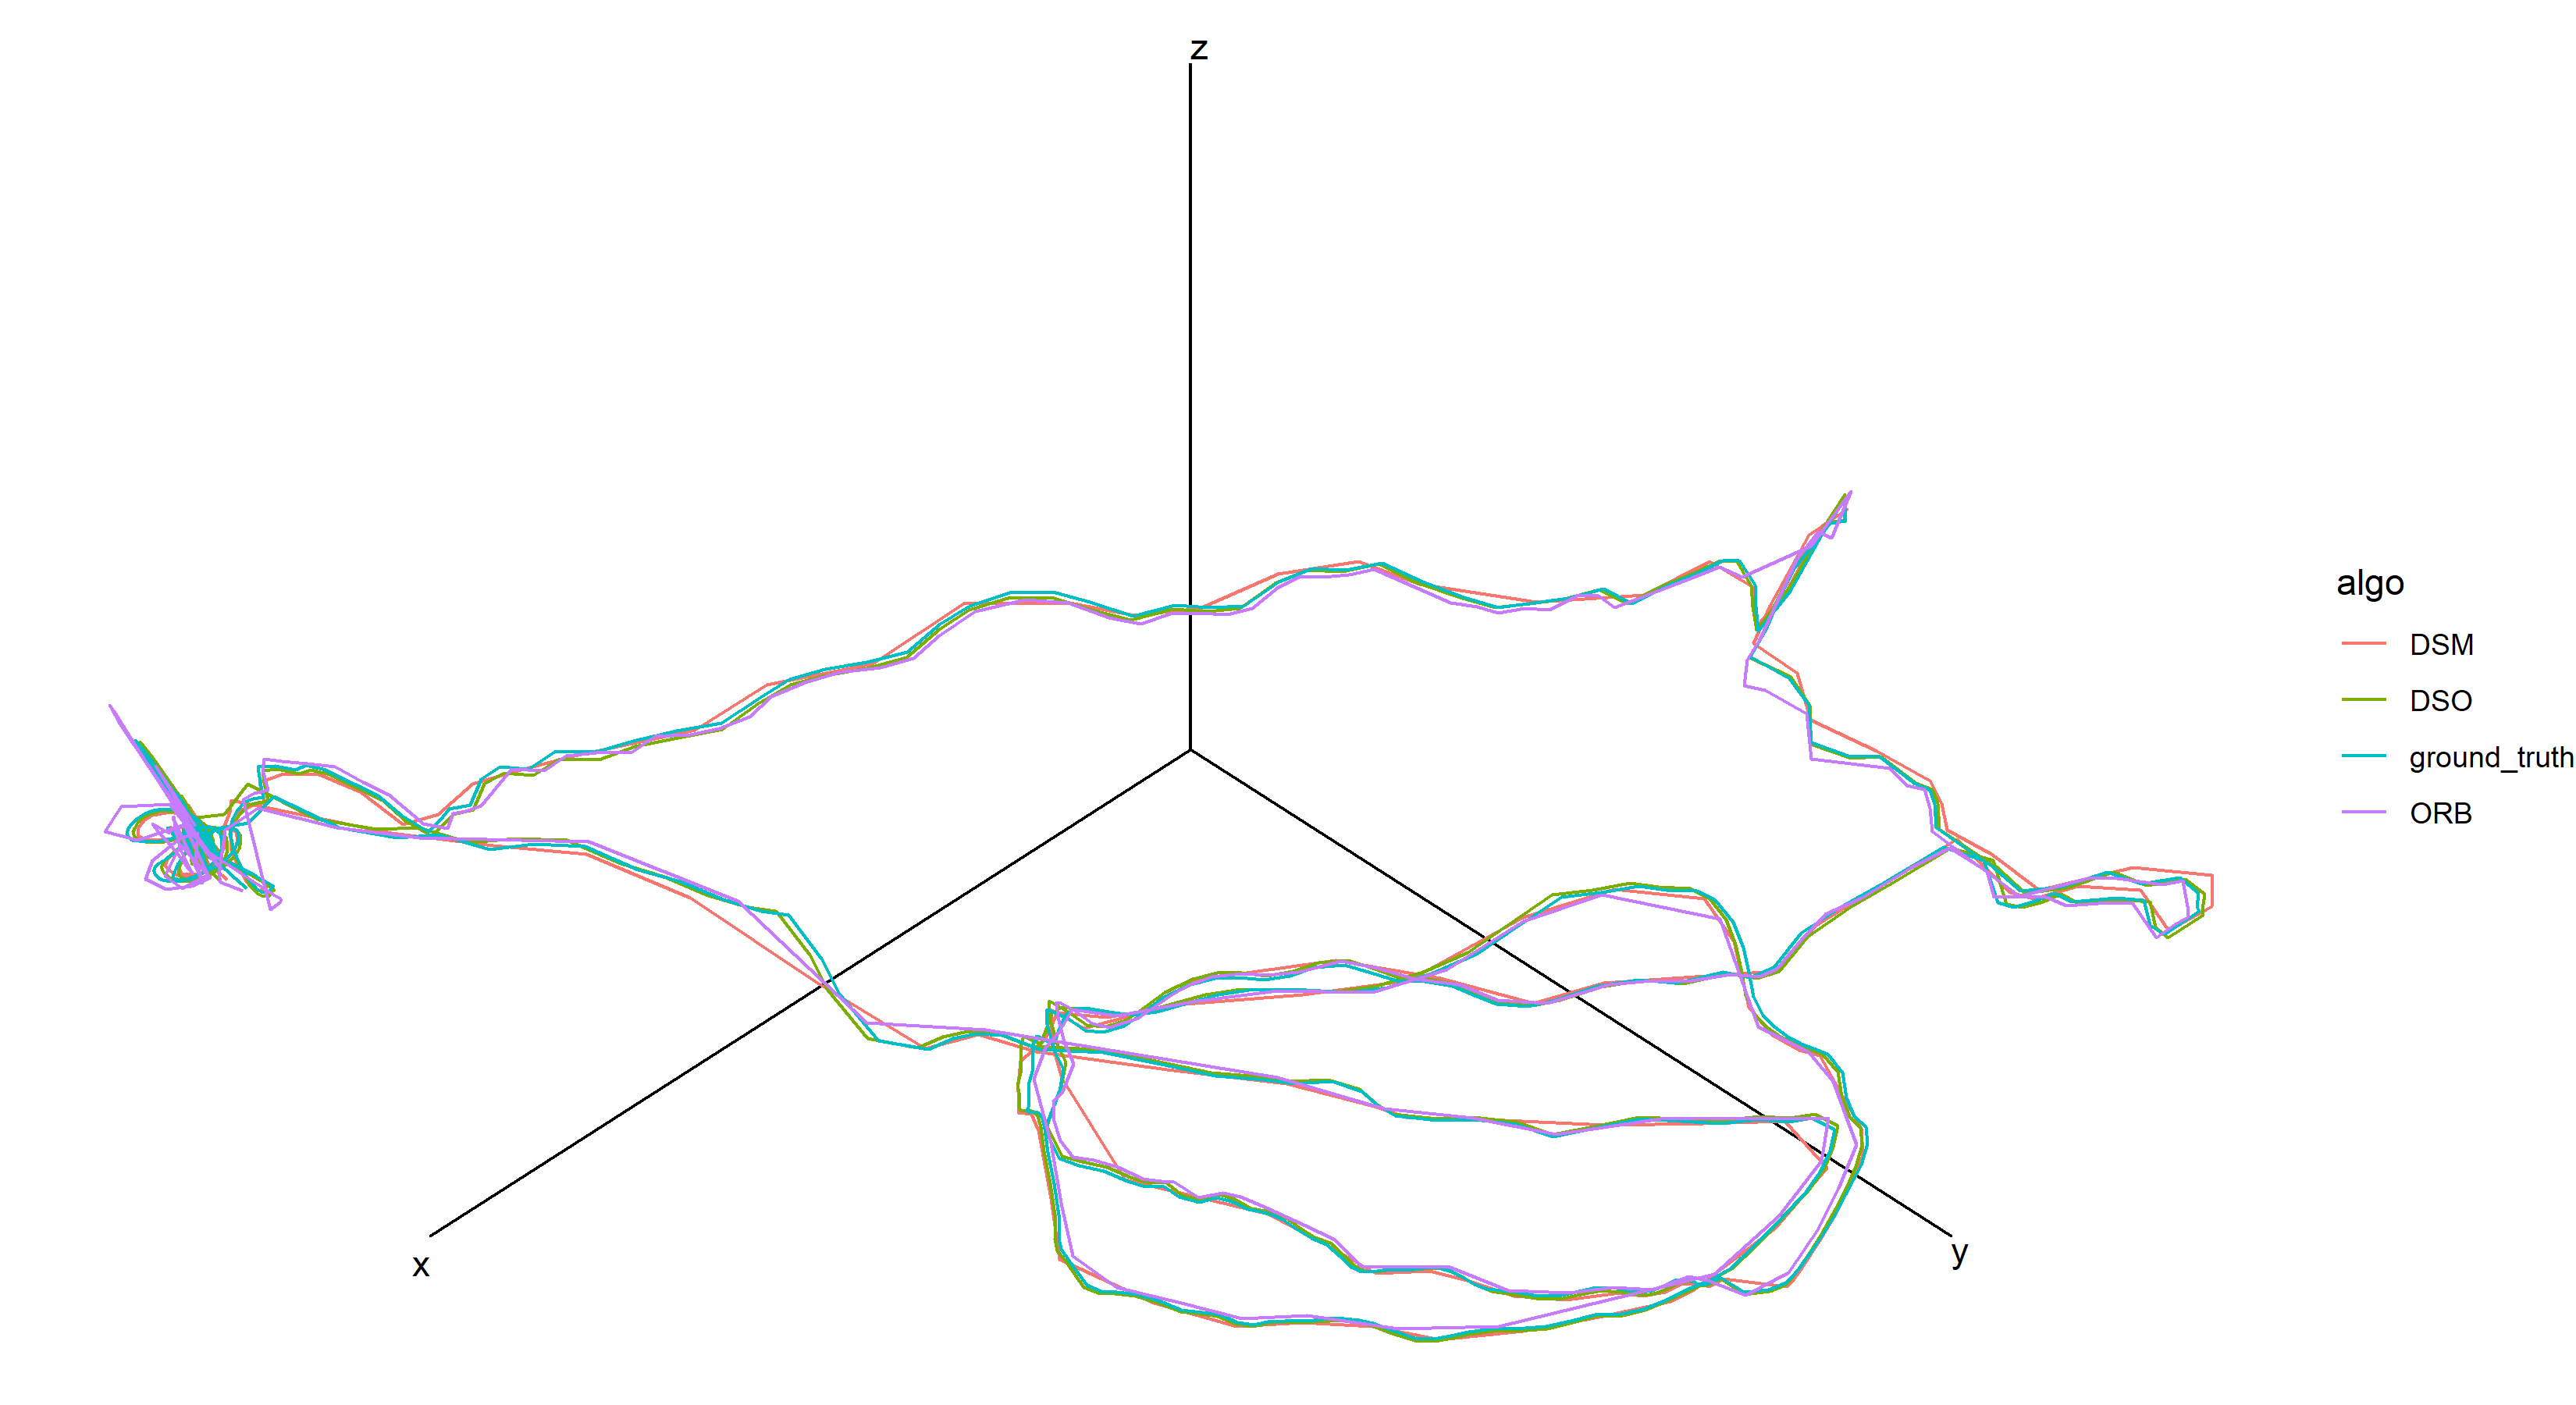
\includegraphics[width=9cm]{img/traj_perf.png} }}%
    \qquad
    \subfloat[\centering V102]{{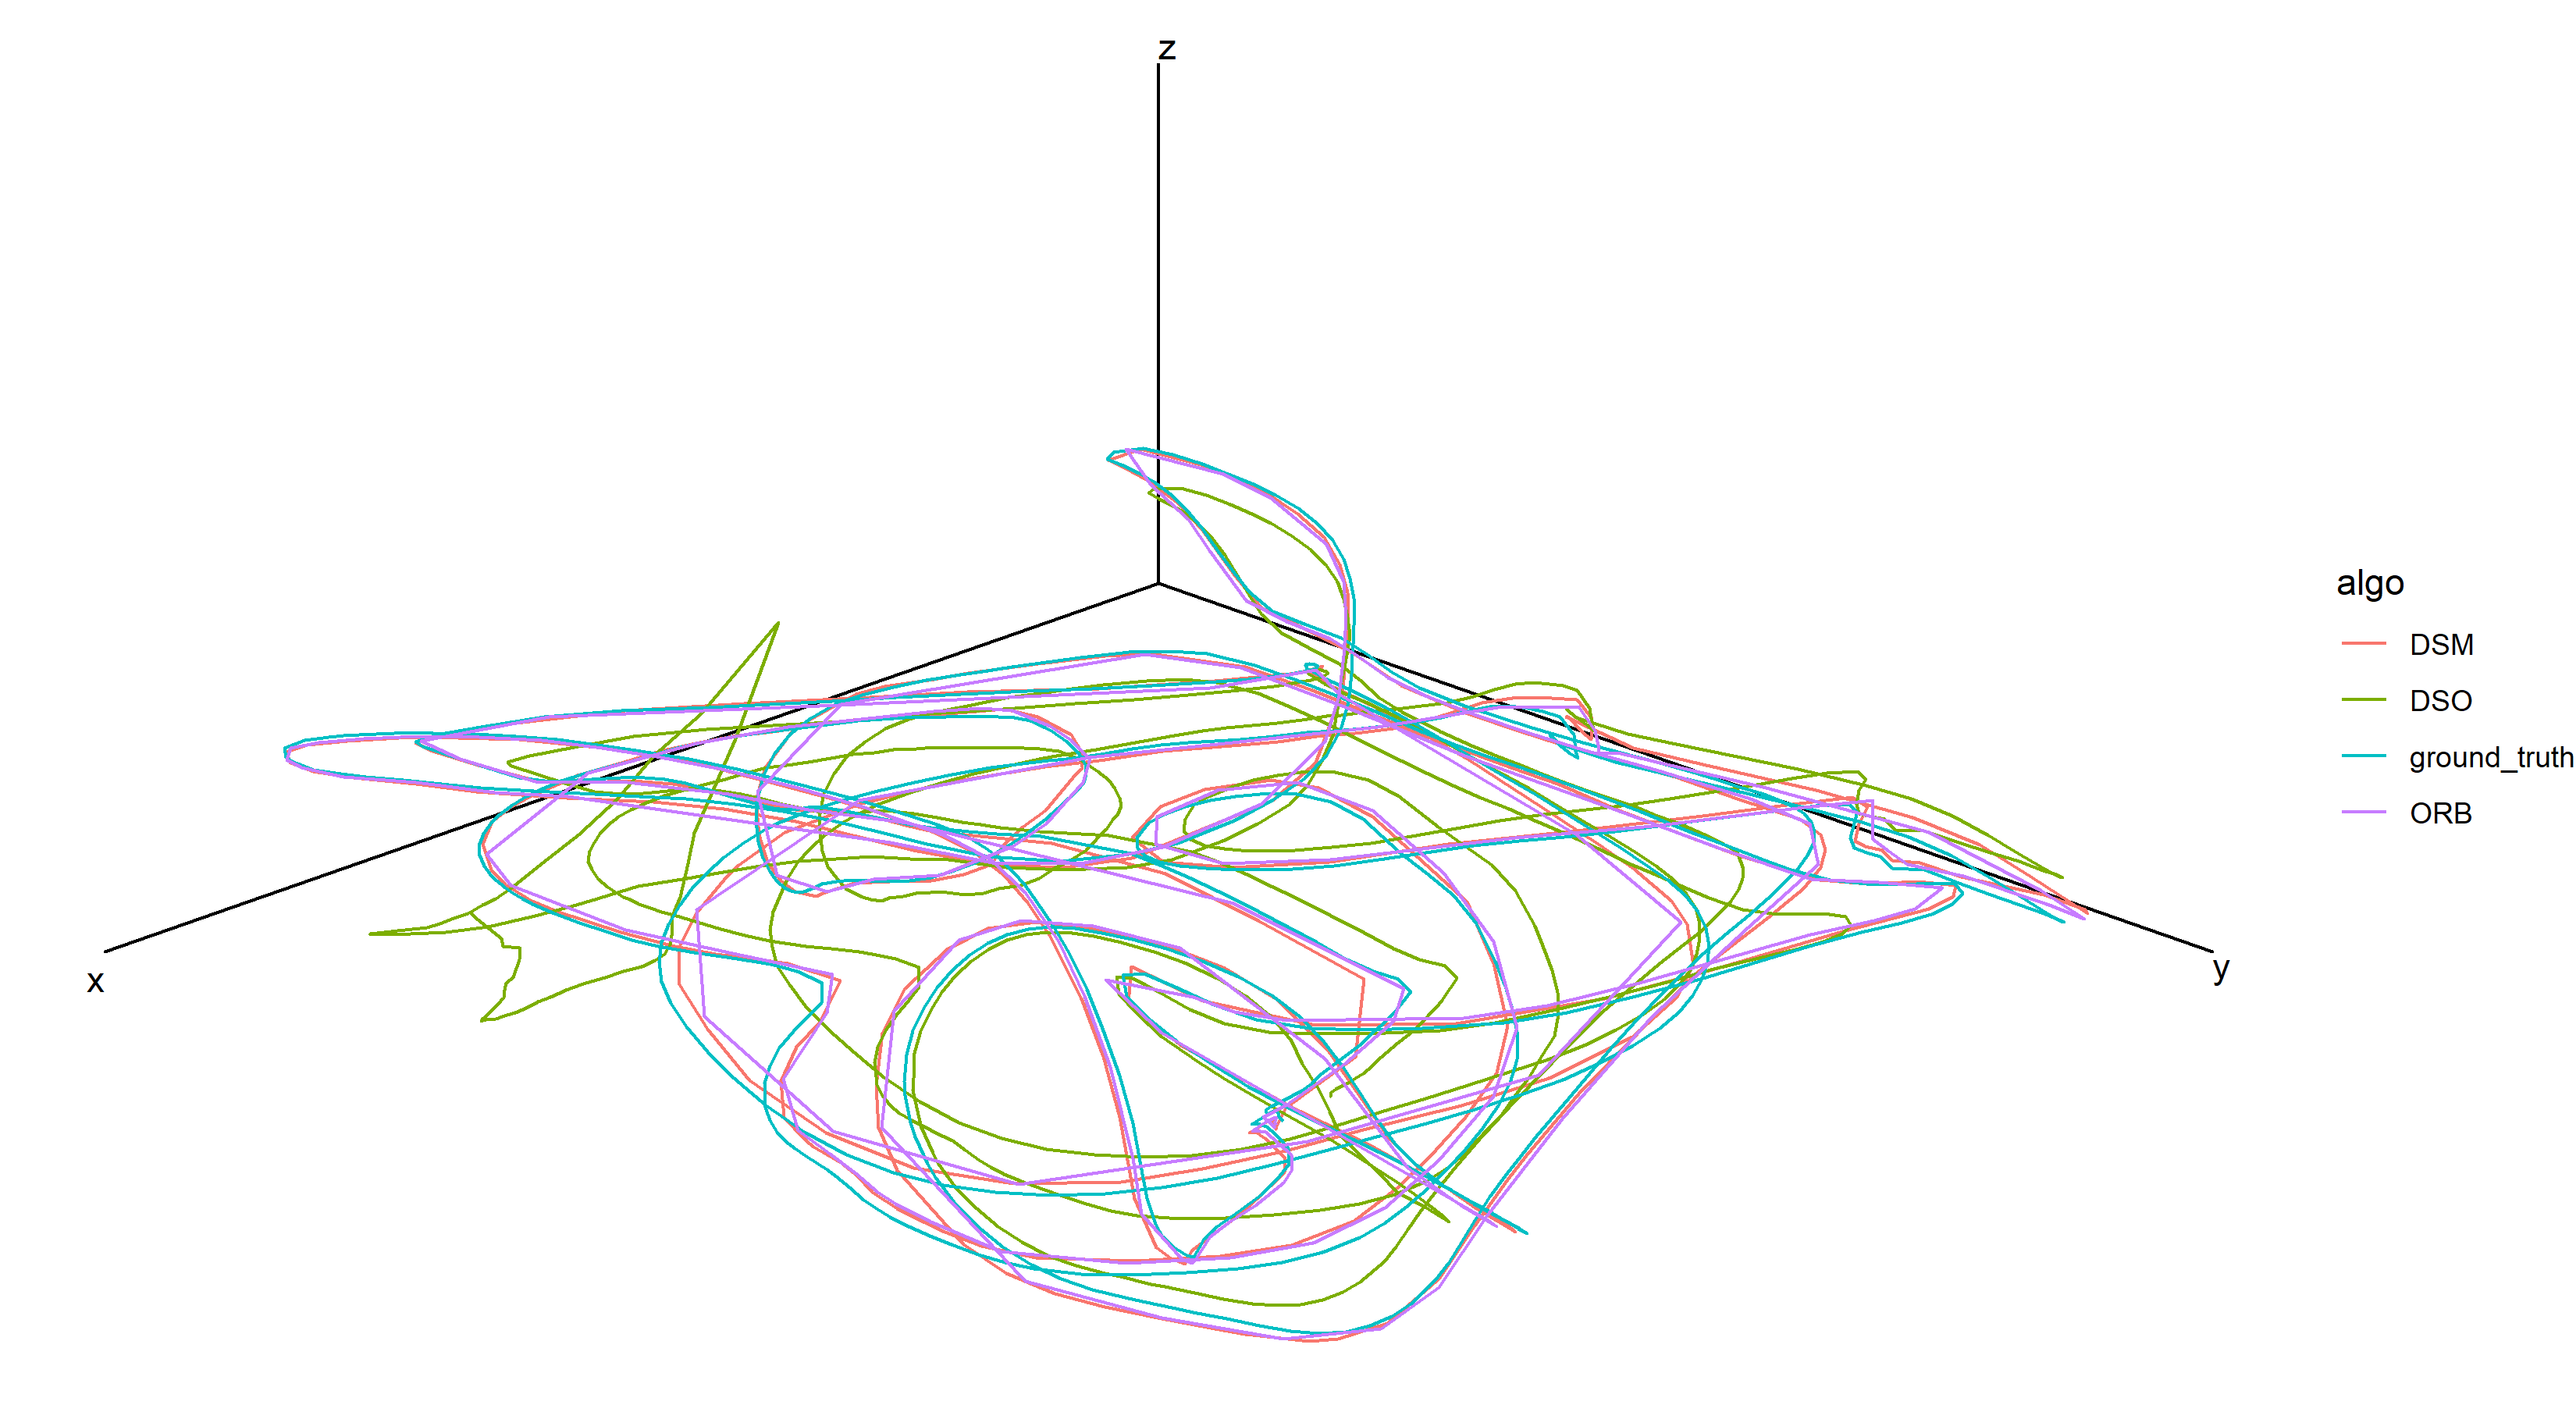
\includegraphics[width=9cm]{img/traj_dso.png} }}%
	\qquad
    \subfloat[\centering V203]{{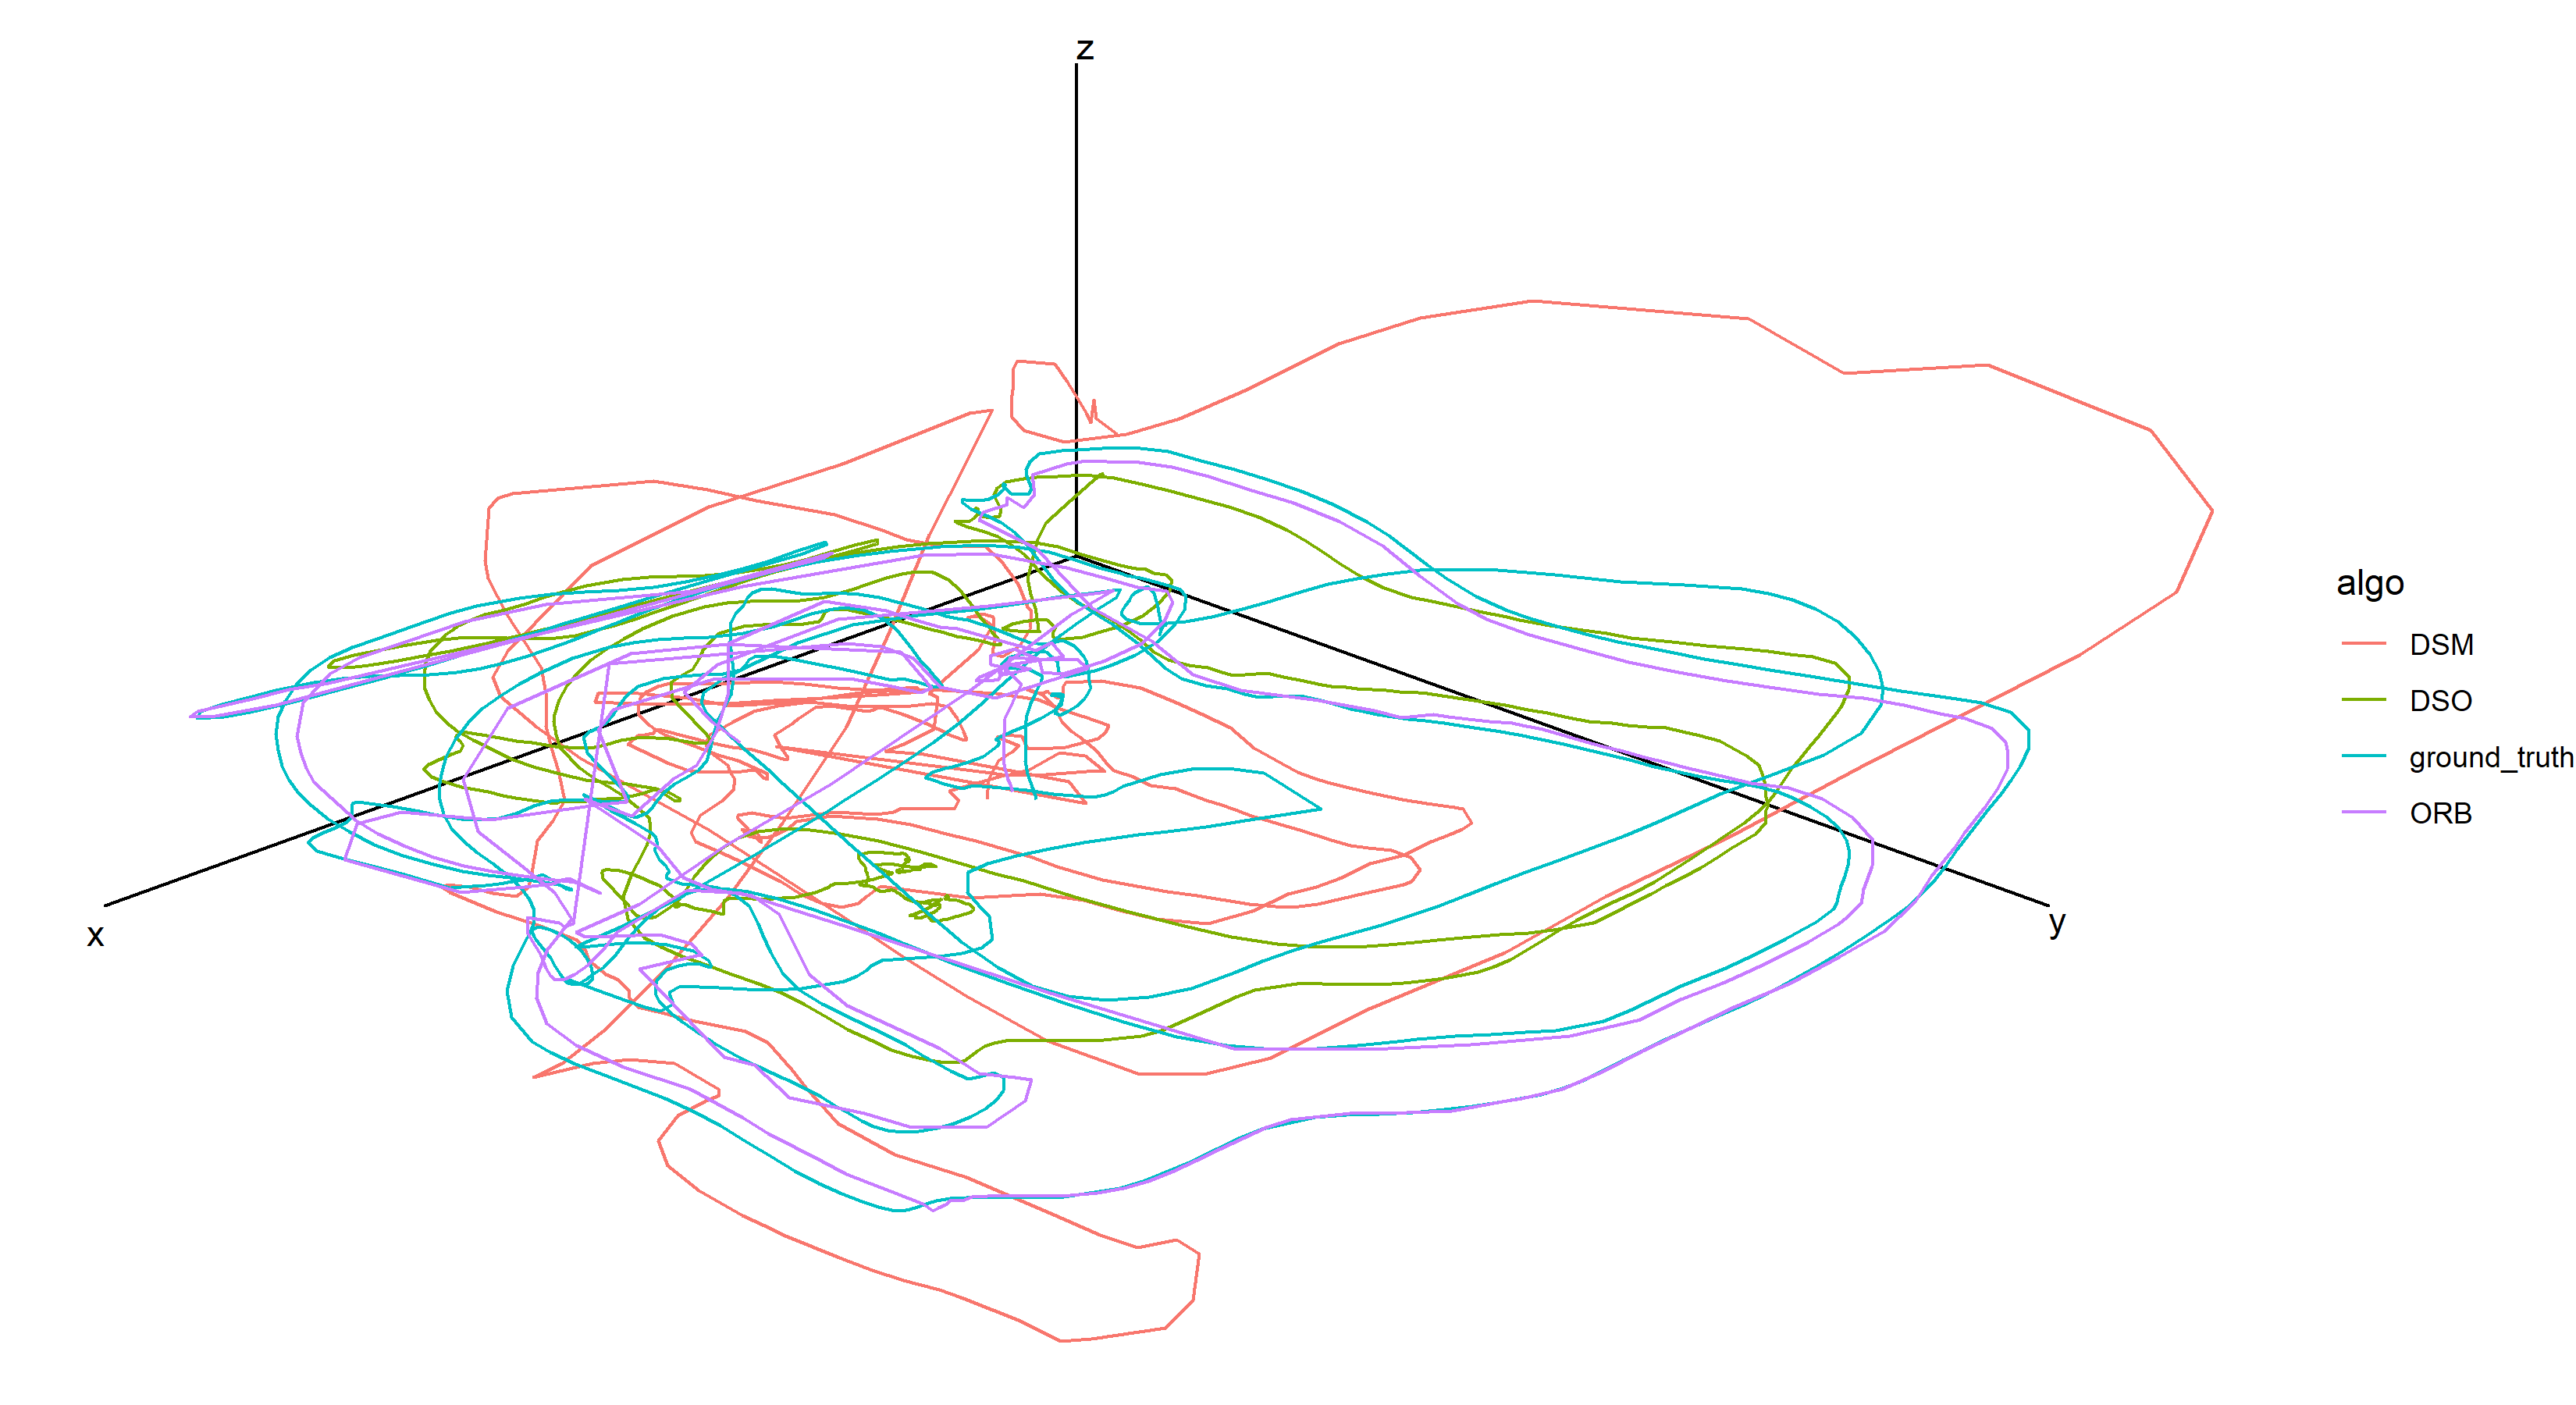
\includegraphics[width=9cm]{img/traj_last.png} }}%
    \caption{
	Ground truth flight path and evaluated flight path of each algorithm after alignment with the method of Umeyama in all axes in meters. 
	Top the sequence MH01, middle the sequence V102 and bottum the sequence V203 are displayed.
	}%
    \label{fig:flight_path}%
	\end{figure}
	
	In figure \ref{fig:flight_path} the computed trajectories are plotted against the ground truth for sequences MH01, V102 and V203 by inserting the 
	trajectories into a 3D coordinate system. This is displayed for the first run only, in order to provide an overview. These sequences 
	were selected, because they represent the results of the visual analysis well. In the first sequence, MH01, all algorithms showed excellent results. 
	One reason for this could be, that in the first sequence, the camera only does very gentle movements, moving at an average speed of $0.41 ms^{-1}$. 
	
	The second image shows the sequence V102. Here, ORB SLAM and DSM SLAM show good results, since in most parts, the trajectories are aligned with the ground truth trajectory.
	DSO SLAM on the 
	other hand shows a significant difference in the flight path. When observing the trajectory closely, the assumption is raised, that the algorithm lost tracking 
	and therefore computed significant wrong position data. This might have caused the calculated positions in the left of the plot, that have a large distance to 
	the ground truth. The rest of the sequence might have been correctly estimated, however since the alignment is done minimizing the term \ref{alignmin}, one significant 
	mistake in the position estimation, might result in severely wrong results over the entire sequence after alignment. This is supported by watching the algorithm running
	and by the fact that in the plot the trajectory looks very similar to the ground truth trajectory, only transformed.
	
	The last plot shows the results of the last sequence. Here, all algorithms had problems estimating a position that comes close to the ground truth position. ORB
	SLAM still showed acceptable performance. However, as described, ORB only tracks about 83 percent of the whole sequence. 
	
	\fig{img/dist_error.png}{Boxplot of the mean positional errors of the runs for each sequence and algorithm}{fig:pos_error}{1}
	
	Furthermore, the euclidean distances between position of the keyframe and the true position of the latter are computed. For a keyframe, 
	the entry of the ground truth data with the lowest distance in time to the time the keyframe was inserted is taken as reference point. 
	This is justifiable, since the true position is sampled at a frequency of over 200 points per second. 
	
	Figure \ref{fig:pos_error} shows the mean distances of all runs for all sequences and for all algorithms. As suspected, in the first five sequences in the machine 
	hall all algorithm performed good. The availability of more features in the scenery and the slow motions of the camera might explain the yielding of these excellent results. 
	Also, as it can be derived in figures \ref{fig:comp2} and \ref{fig:comp1}, DSO SLAM tends to drift further apart from the ground truth position the longer the tracking is active. 
	This might be the result of lacking the functionality to close loops and to optimize over the global map, as explained in section \ref{samemodel} . 
	
	To summarize, over all runs and sequences, including the sequences, where the tracking was lost, ORB SLAM had a positional difference to the ground truth 
	of 11 cm, DSO SLAM of 32cm and DSM SLAM of 17cm. When excluding sequence V103 and V203, ORB evaluated the position with an average error of 7cm, DSO SLAM with 17cm and DSM SLAM with 6cm. 
	
\subsection{Point Cloud Evaluation}

For the evaluation of the computed point clouds, these point clouds were first visually observed, as described in section \ref{pceval}. 
Figure \ref{fig:pointcloud} shows the evaluated point clouds aligned with the ground truth point cloud for sequence V101. In this sequence
 the tracking of the trajectory was successfull for all three algorithms, thus, the errors of the resulting point clouds can not 
be a result of errors in alignment. 

What becomes clear at the first glance is that ORB SLAM generates only few points, since only found keypoints are mapped in feature-based methods.
 To give these  points better visibility, the point size was doubled in the ORB image. DSM- and DSO SLAM generate point clouds with significant higher 
 density, where all structures of the room are immediately visible with good quality. 
 
 On the other side, the advantage of ORB-SLAM over the other two direct methods 
 is the recognition of clear features in terms of structural differences in the scenes. Though DSO- and DSM SLAM also regard the differences in the pixel intensities, ORB SLAM detects the features on different scale levels and ensures that the regarded features are truly significant, as described in section \ref{orbcomp}.
 This also became clear when observing the point cloud. All significant features, and therefore important features for autonomous navigation, were successfully 
 marked with a computed point. For example, this can be seen at the ladder in the third image of figure \ref{fig:pointcloud}, where all the subsequent rungs contain at least 
 one point. 
 
 After elaboration on the point clouds, it also became clear, that the point clouds of DSO, often generate point clouds, where multiple layers of 
 points were falsely generated and all points had the same clear distance to the ground truth point cloud. This may be a result of the functionality of DSO slam, 
 where marginalized keyframes are removed permanently. For revisited areas, the points are regenerated. This means that all errors made
 in the sequence accumulate and when an area is revisited, significant errors in the point cloud can occur. This can be seen when looking at the 
 third image closely. When looking at the mattress in the middle of the room, the accumulated error expresses itself by points hovering in the air 
 in a clear plane. 

	\begin{figure}%
    \centering
    \subfloat[\centering ORB]{{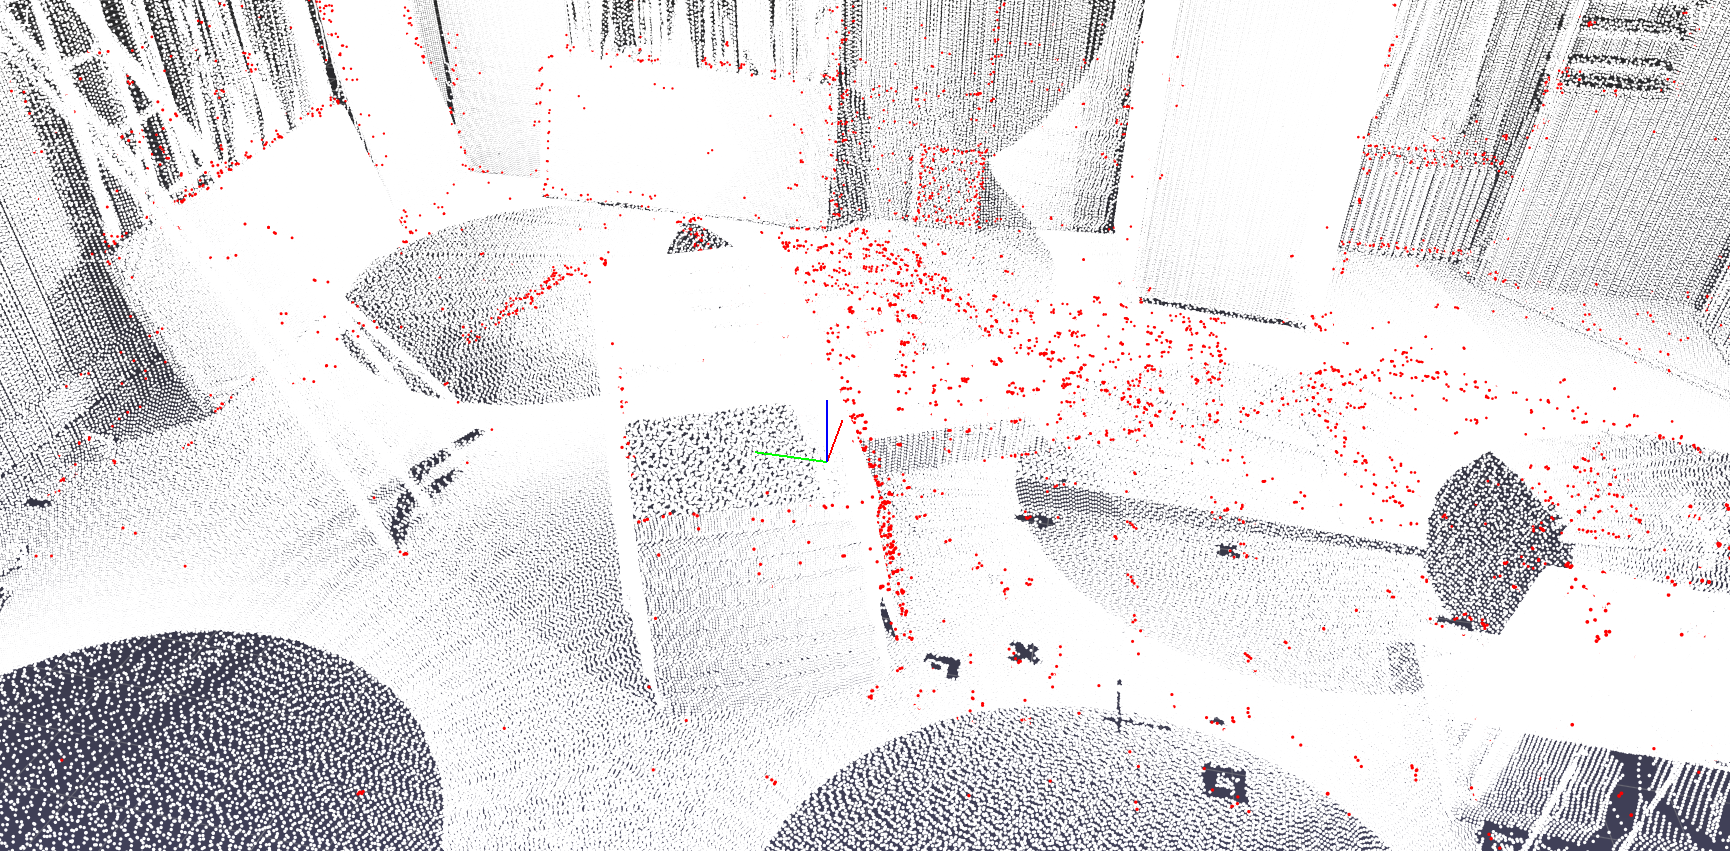
\includegraphics[width=7cm]{img/pointcloud_orb} }}%
    \qquad
    \subfloat[\centering DSM]{{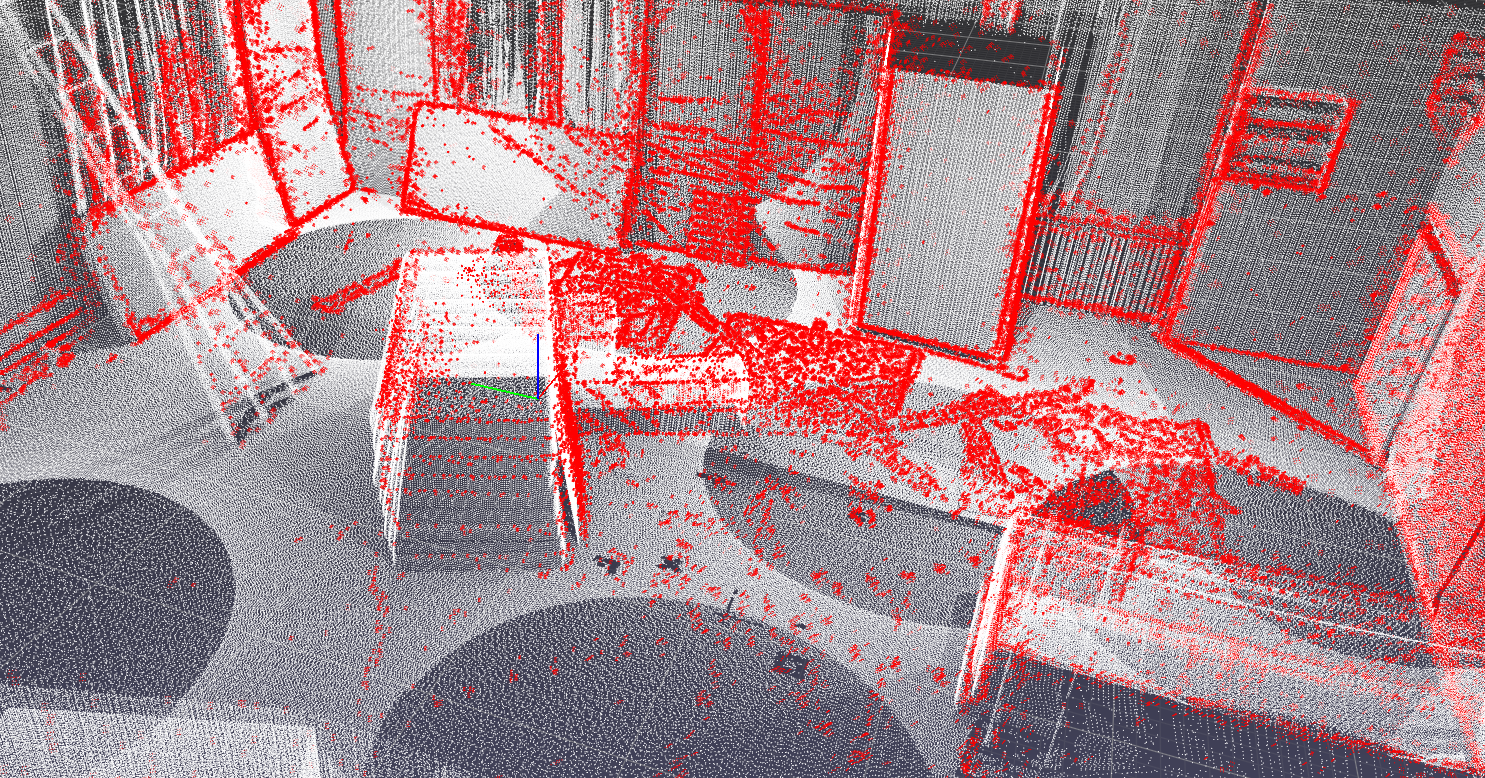
\includegraphics[width=7cm]{img/pointcloud_dsm} }}%
	\qquad
    \subfloat[\centering DSO]{{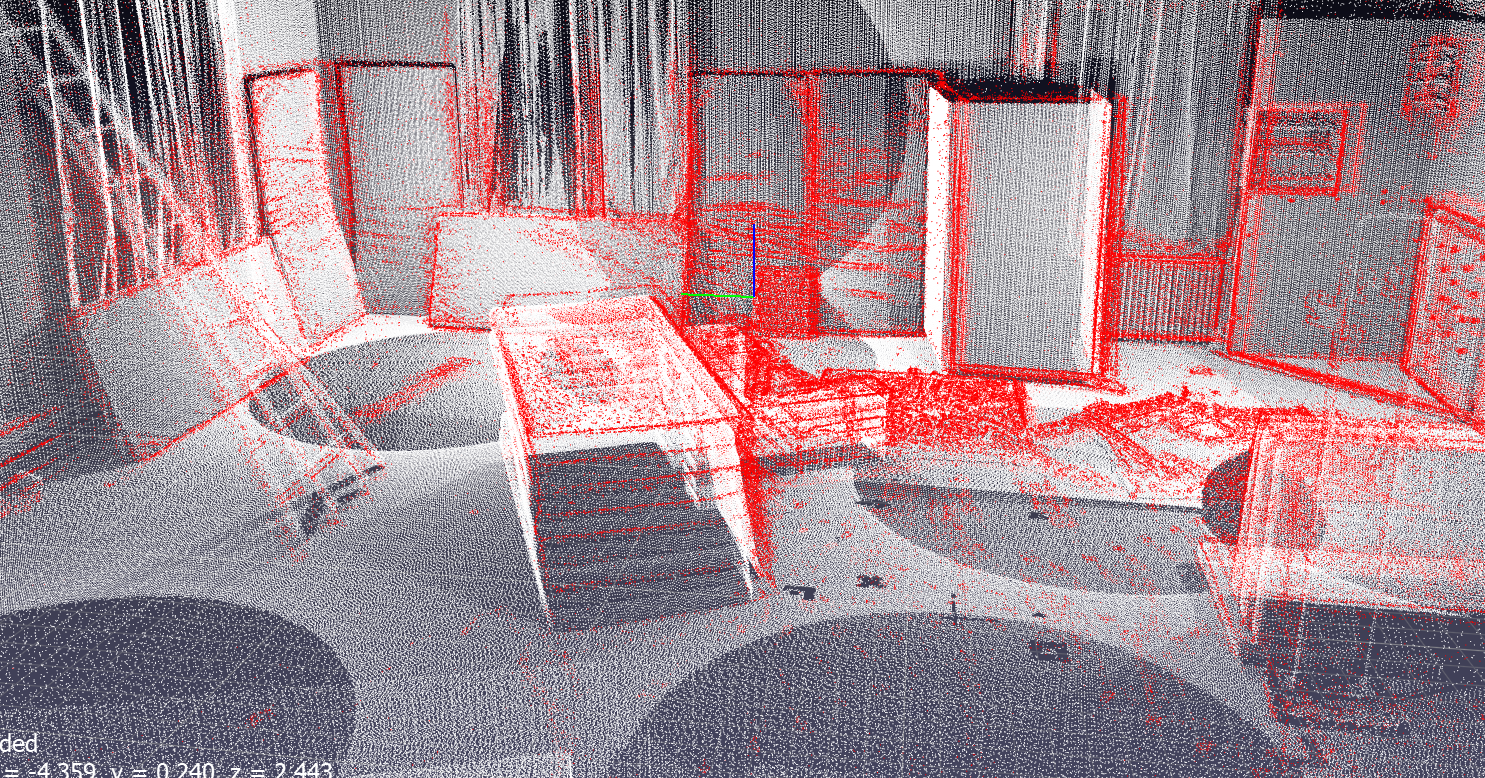
\includegraphics[width=7cm]{img/pointcloud_dso} }}%
    \caption{The ground truth of the point cloud from Sequence V101 (white points) and the evaluated points by each algorithm (red points). 
	The points in Figure (a) are twice as large for better visibility (ORB-SLAM generates only few points). 
	}%
    \label{fig:pointcloud}%
	\end{figure}
	
	
	The density can also be expressed by numbers. The significant difference of the numbers of points can be seen in table \ref{table:pointcloud}. While 
	ORB SLAM only generates close to 10000 points in the sequences, DSM SLAM generates more than 500000 points in most sequences and DSO SLAM more than 200000 
	in most sequences. 
	
	\begin{table}
	\caption{Absolute number of points and mean distance to the closest point in the ground truth point cloud in meter (written in parentheses) for each algorithm and sequence averaged over all runs.}
	\begin{tabular}{ |p{3cm}||p{3cm}|p{3cm}|p{3cm}|  }
	\hline
	Sequence Name& ORB & DSM & DSO \\
	\hline
	MH\_01\_easy & 9959.7 (/) & 683237.3 (/) & 371389.7 (/)\\
	MH\_02\_easy & 9551 (/) & 678000.0 (/) & 342405.7 (/)\\
	MH\_03\_medium & 7652.7(/) & 634178.7 (/) & 372070.3 (/)\\
	MH\_04\_difficult & 10084.3 (/) & 505642.7 (/) & 211698.7 (/)\\
	MH\_05\_difficult & 10607.3 (/) & 505677.3 (/) & 234682.7 (/)\\
	V1\_01\_easy & 8088.3 (0.0418) & 582530.7 (0.0593) & 372805.7 (0.0734)\\
	V1\_02\_medium & 7927.3 (0.0486) & 642992.0 (0.0672) & 356028.7 (0.6028)\\
	V1\_03\_difficult & 9373.7 (0.3137) & 786626.7 (0.0955) & 445751.0 (0.6416)\\
	V2\_01\_easy & 10154.0 (0.0515) & 589416.0 (0.0736) & 244025.7 (0.0927)\\
	V2\_02\_medium & 9007.7 (0.0509)& 785309.3 (0.1557) & 494689.7 (0.0976)\\
	V2\_03\_difficult & 10985.7 (0.4350) & 831517.3 (0.7208) & 464663.3 (0.6189)\\
	\hline
	\end{tabular}
	\label{table:pointcloud}
	\end{table}
	
	However, regarding the accuracy of the computed points by the algorithms, again ORB SLAM shows the best performance. In table \ref{table:pointcloud}, 
	for all sequences, where a ground truth point cloud exists, the distance to the closest point in the ground truth point cloud is computed by randomly sampling
	150 points per algorithm and sequence. The means of each run again averaged an shown in table \ref{table:pointcloud}. 
	
	\fig{img/pq_dist.png}{Boxplot of the means for each run of the euclidean distances between an evaluated point and the closest point of the ground truth point cloud.
	For computational feasibility, for each sequence, run and algorithm, 150 points for evaluation are sampled randomly}{fig:boxplot_pq}{1}
	
	The result is also shown in figure \ref{fig:boxplot_pq}, where the correlation between the trajectory accuracy and the point cloud accuracy become clearly 
	visible. Averaged over all runs and sequences, a point generated by ORB SLAM lies 15cm from the next ground truth point, DSM SLAM 19cm and DSO SLAM 35cm. 
	Unlike the trajectory error, the point cloud error of ORB SLAM is still the smallest when the Sequences V103 and V203 are not considered. Then ORB SLAM 
	only causes an error of 4.8cm, DSM of 8.8cm and DSO of 21cm. This is because ORB SLAM does not generate as many outliers as DSO- and DSM SLAM, as it can be seen 
	in figure \ref{fig:distr}.
	
	\fig{img/pc_distr.png}{Distribution of the error distances of Sequence V101 and run 1.}{fig:distr}{1}
	
	

\subsection{Computation Time}

	The computation time for each sequence and algorithm was measured, respectively the time the algorithm consumed to complete the computation of the sequence.
	
	In order to evaluate, if an algorithm can run in realtime, the absolute times have to be broken down into the computed frames per second.
	The EuRoC dataset consists of sequences recorded at a frame frequency of 20 frames per second. This means the total frames per sequence 
	amount to the duration of sequence in seconds times 20. For the computed frames per second, this value is then divided by the time the algorithm needed 
	to process the sequence. 
	
	The results are displayed in table \ref{table:comp_time}. ORB SLAM processes the frames at a frame per second rate of 17, 
	DSM SLAM processes the frames at 4.17 frames per second and DSO SLAM at a rate of 5.22. Thus, 
	none of the evaluated SLAM algorithms processes any of the evaluated sequences in realtime, but ORB SLAM is at least 
	three times as fast as both other algorithms in processing the frames. 
	
	\begin{table}
	\caption{Computation time (excluded time needed for initialization) of each sequence and algorithm, averaged over all runs. In parentheses the 
	resulting computed frames per second are given.}
	\begin{tabular}{ |p{3cm}||p{3cm}|p{3cm}|p{3cm}|  }
	\hline
	Sequence Name & Computation Time in $s$ ORB & Computation Time in $s$ DSM & Computation Time in $s$ DSO \\
	\hline
	MH\_01\_easy & 215 (17.0) & 688 (5.30) & 798 (4.56)\\
	MH\_02\_easy & 174 (17.2) & 538 (5.57) & 732 (4.10)\\
	MH\_03\_medium & 157 (16.9) & 656 (4.02) & 403 (6.85)\\
	MH\_04\_difficult & 117 (16.9) & 394 (5.02) & 260 (7.69)\\
	MH\_05\_difficult & 132 (16.8) & 385 (5.76) & 372 (5.97)\\
	V1\_01\_easy & 168 (17.1) & 612 (4.71) & 628 (4.58)\\
	V1\_02\_medium & 101 (16.6) & 678 (2.46) & 345 (4.99)\\
	V1\_03\_difficult & 123 (17.1) & 907 (2.32) & 654 (3.22)\\
	V2\_01\_easy & 131 (17.1) & 461 (4.87) & 357 (6.28)\\
	V2\_02\_medium & 136 (17.0) & 783 (2.95) & 415 (5.55)\\
	V2\_03\_difficult & 133 (17.1) & 796 (2.89) & 640 (3.60)\\
	\hline
	\end{tabular}
	\label{table:comp_time}
	\end{table}

